\documentclass[12pt,a4paper]{article}
\usepackage[top=2.5cm,bottom=2.5cm,left=2.2cm,right=2.2cm]{geometry}
\usepackage{polski}
\usepackage[utf8]{inputenc}
%%\usepackage[OT4]{fontenc}
\usepackage{amsmath,amsfonts,amssymb,amsthm}
\usepackage{enumerate}
\usepackage{url}
\usepackage{multicol}
\usepackage{color}
\usepackage{graphicx} 
\usepackage{setspace}
\usepackage{float}
\usepackage{subfig}
\usepackage{listings}
\usepackage{pythonhighlight}
\usepackage{lipsum}
\usepackage{tabularx}
\usepackage{hyperref}

%\pagestyle{empty}
%WYMIARY STRONY
\topmargin -30mm
\oddsidemargin -1.7cm
\evensidemargin -1.7cm
\textwidth 180mm
\textheight 260mm
%\usepackage{psfrag}

\usepackage{amsmath}
\usepackage{amsfonts}

\usepackage{supertabular}
\usepackage{array}


\usepackage{tabularx}
\usepackage{hhline}

\newcommand{\myand}{i\ }
%\usepackage{showlabels}

\newcommand{\R}{I\!\!R} %symbol liczb rzeczywistych, dzia³a tylko w
                        %trybie matematycznym
\newtheorem{theorem}{Twierdzenie}[section] %nowe otoczenie do
                                           %sk³adania twierdzeñ

\usepackage{titlesec}
\titleformat*{\section}{\normalsize\bfseries}
\titleformat*{\subsection}{\footnotesize\bfseries}
\titleformat*{\subsubsection}{\normalsize}
\title{Klasyfikator oparty o drzewo decyzyjne}
\date{13.03.2018}
\author{Łukasz Odwrot 218283}

%ustawianie marginesów
\usepackage{geometry}
\newgeometry{tmargin=2.5cm, bmargin=2.5cm, lmargin=2.5cm, rmargin=2.5cm}


 
 
\begin{document}
\maketitle
\thispagestyle{empty}
\newpage
\tableofcontents
\setcounter{page}{1}
\newpage

\section{Wstęp}
Naiwny klasyfikator bayesowski to prosty klasyfikator probabilistyczny oparty o twierdzenie Bayesa i założeniu o niezależności zmiennych losowych.  Dla danej klasy obiektu y i wektora cech X na podstawie twierdzenia Bayesa prawdziwy jest wzór:


$$ P(y\mid x_{1},..., x_{n}) = 
\frac
{P(y)P(x_{1},...x_{n}\mid y)}
{P(x_{1},...,x_{n})}
$$

Korzystając z założenia o niezależności zdarzeń i przekształceń można dojść do wzoru:

$$  \hat{y} = arg \max_{y} P(y) \prod_{i=1}^{n} P(x_{i} \mid y) $$

Dzięki takiemu mechanizmowi na podstawie ciągu uczącego można wytrenować klasyfikator, a następnie wykorzystać go do klasyfikacji nowych obiektów. Do badania jakości uzyskanych klasyfikatorów użyte zostaną następujące mechanizmy: Confusion Matrix, ccuracy, Precision, Recall, Fscore. Badania zostaną przeprowadzone na trzech zbiorach danych: Glass, Wine oraz Diabetes.

\section{Badane zbiory}

Rozkłady cech dla poszczególnych klas przedstawiono na poniższych rysunkach.

\begin{figure}[H]
\centering
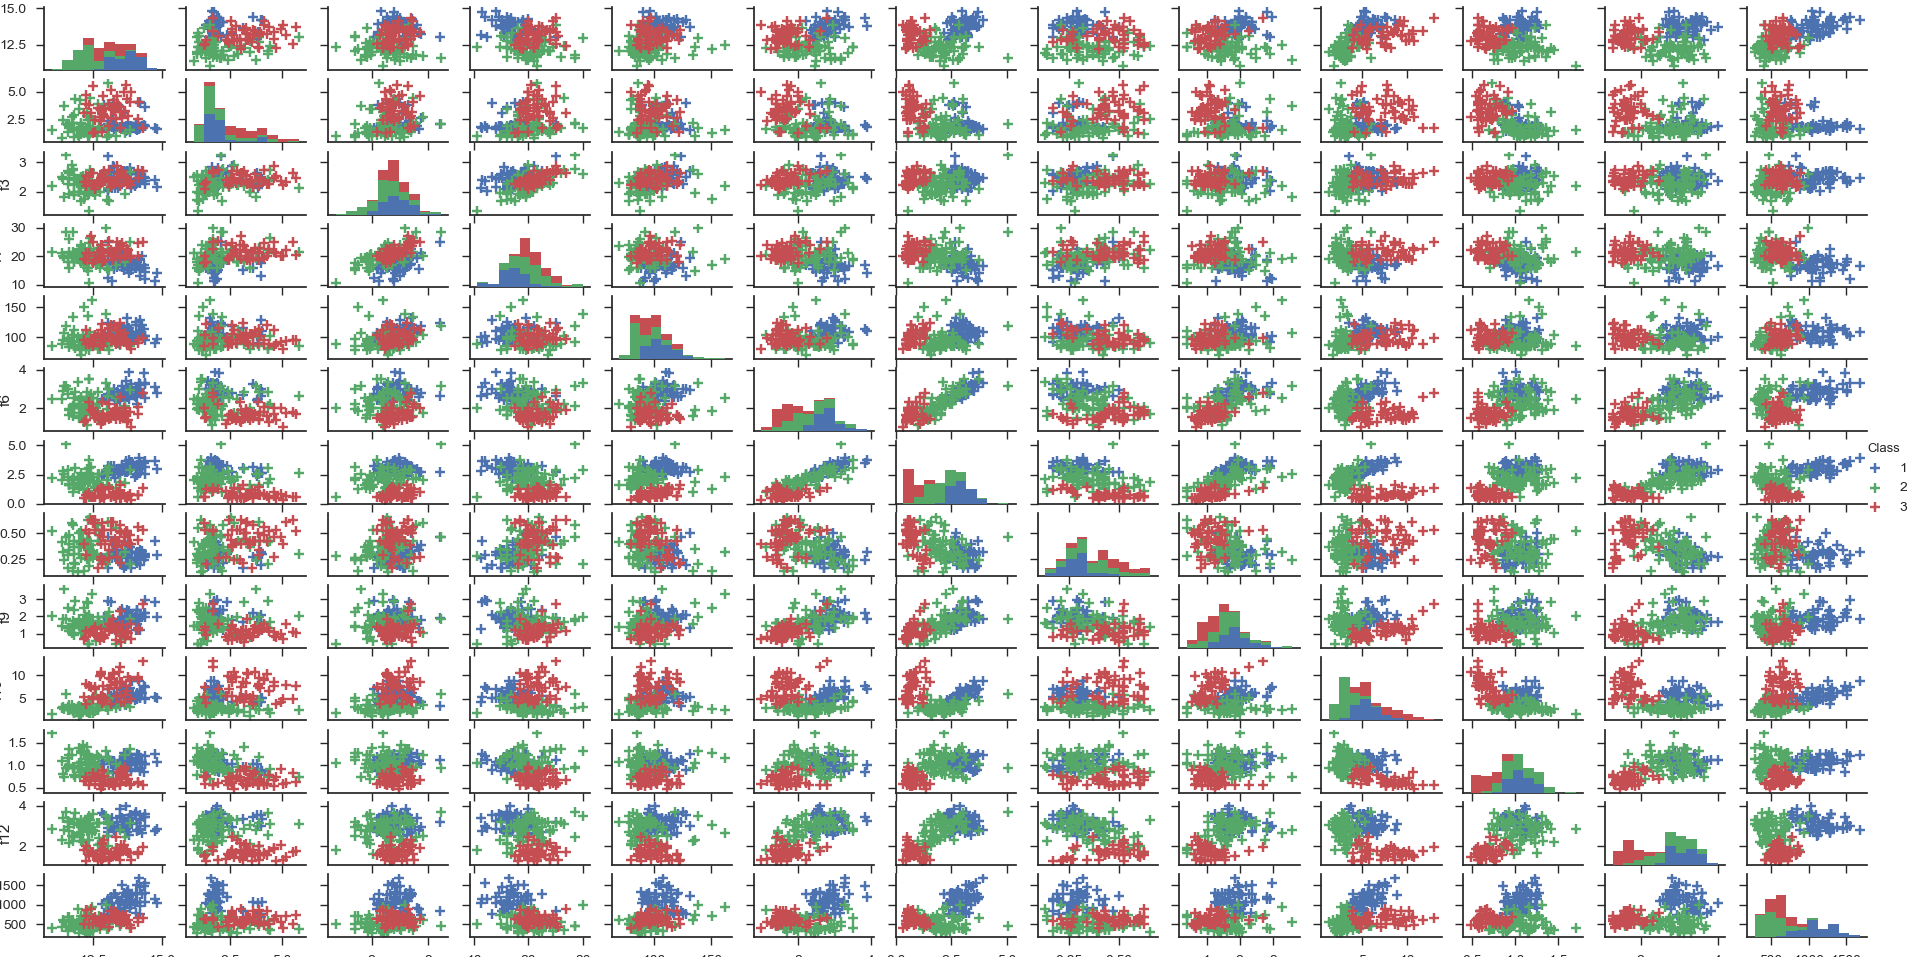
\includegraphics[width=1\textwidth]{dsWineCombined.png}
\caption{Rozkład cech dla zbioru Wine}
\end{figure}

\begin{figure}[H]
\centering
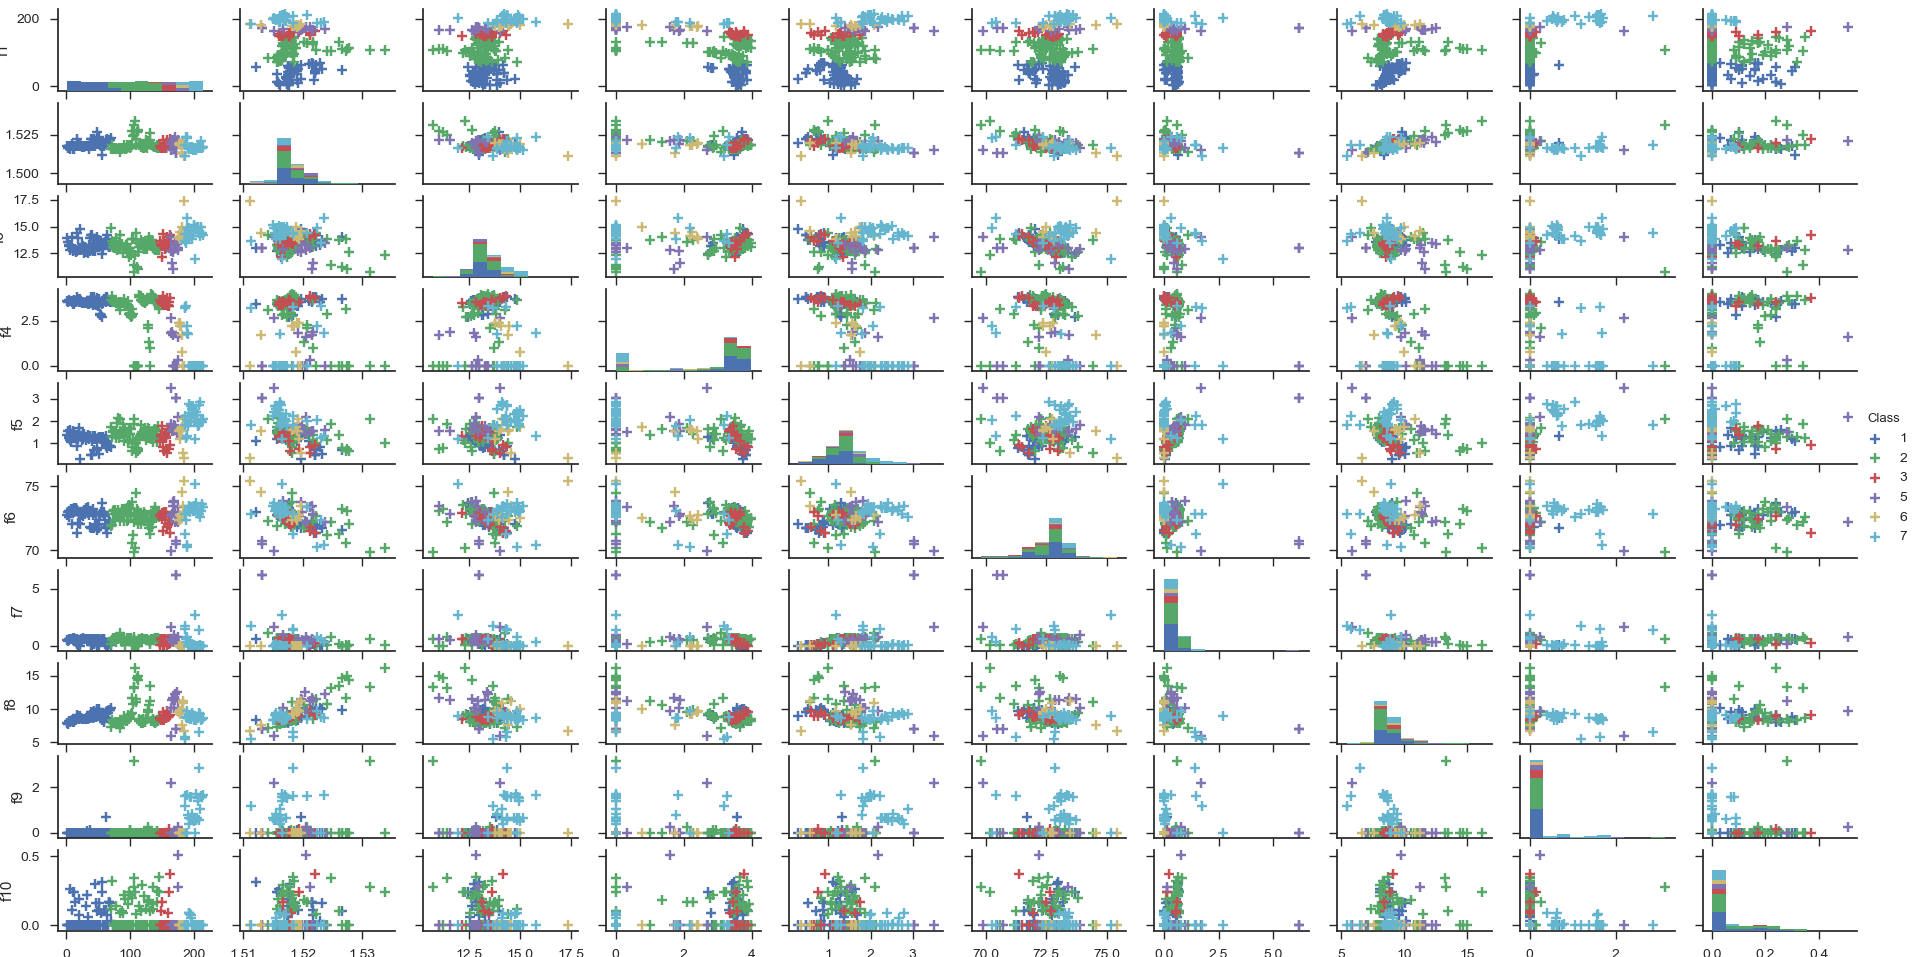
\includegraphics[width=1\textwidth]{dsGlassCombined.png}
\caption{Rozkład cech dla zbioru Glass}
\end{figure}

\begin{figure}[H]
\centering
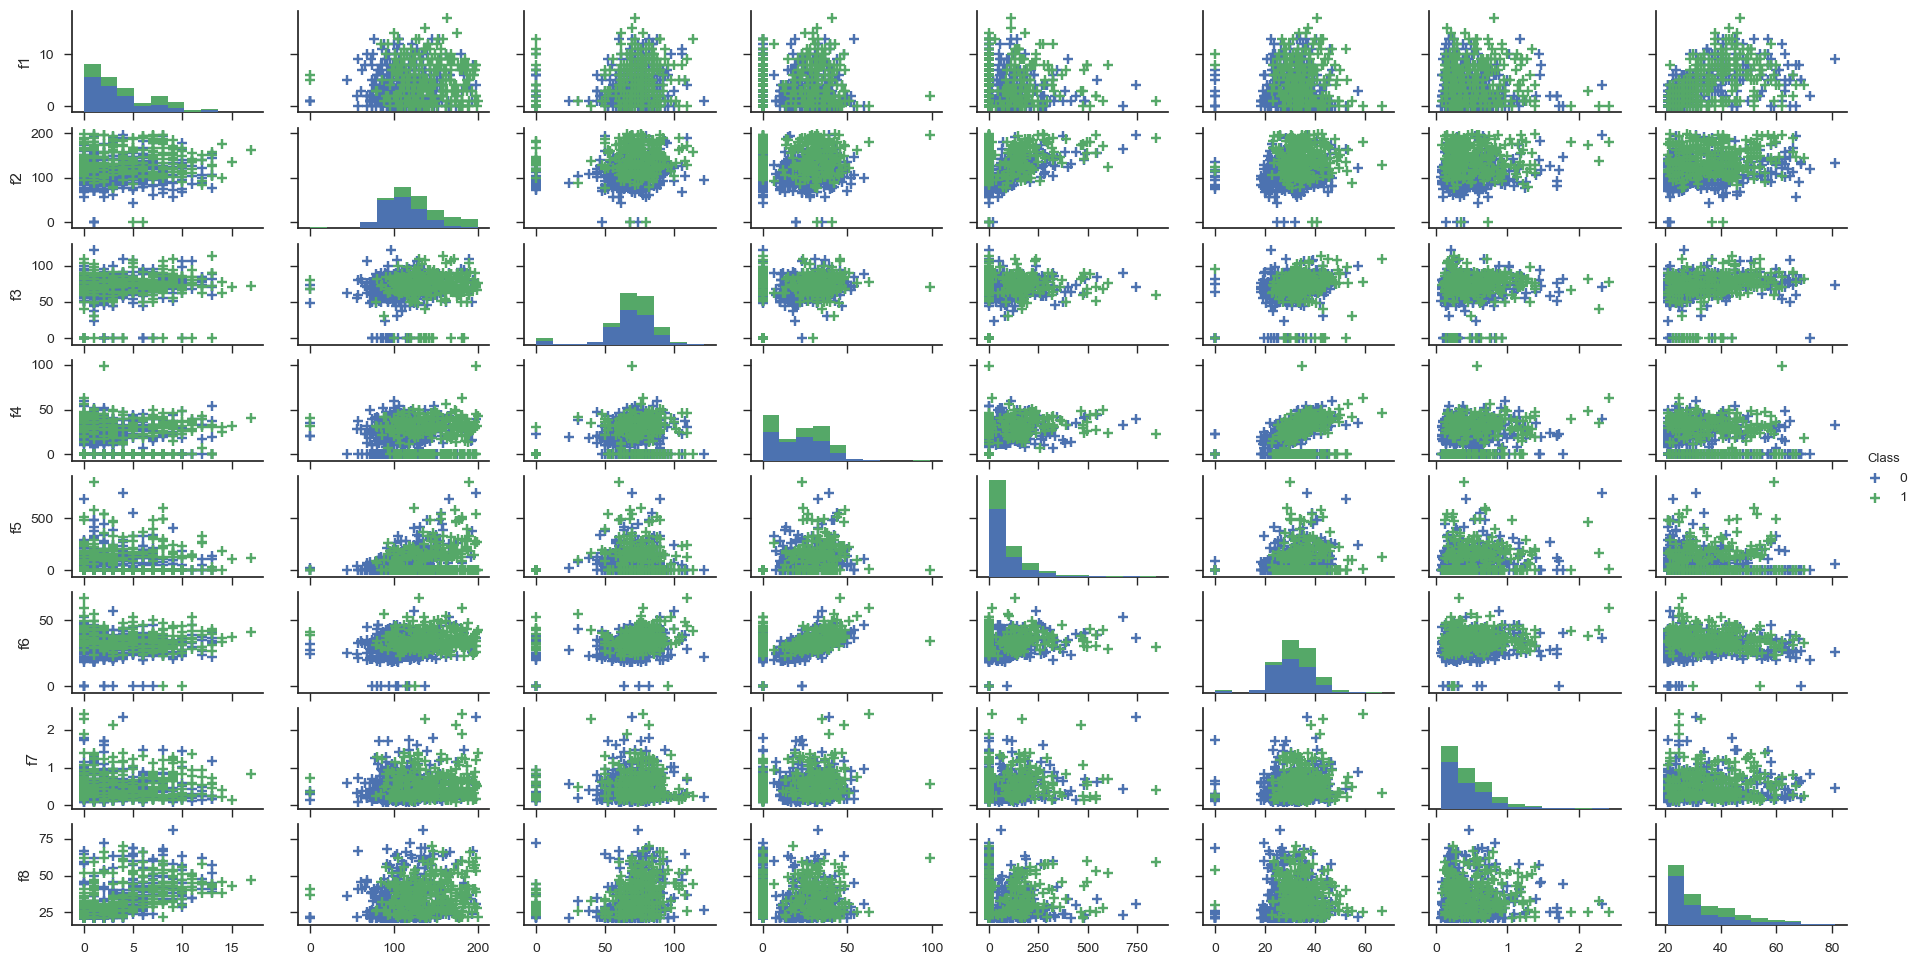
\includegraphics[width=1\textwidth]{dsDiabetesCombined.png}
\caption{Rozkład cech dla zbioru Diabetes}
\end{figure}

\section{Porównanie metod kroswalidacji}
Zaimplementowane zostały dwie metody kroswalidacji:
\\
\textsl{•} Niestratyfikowana (ręcznie)
\\
\textsl{•} Stratyfikowana (z pomocą biblioteki caret)
\\
Do porównania wyników użyty zostanie parametr fscore.







\section{Badane parametry}
Do zbadania wybrano wpływ modyfikacji 4 różnych parametrów na drzewo. Domyślna konfiguracja parametrów drzewa wygląda następująco:
(subset = TRUE, bands = 0, winnow = FALSE, noGlobalPruning = FALSE, CF = 0.25, minCases = 2, fuzzyThreshold = FALSE, sample = 0, seed = sample.int(4096, size = 1) -1L, earlyStopping = TRUE, label = "outcome")

MinCases - określa minimalną ilość próbek w danym liściu.

\begin{figure}[H]
\centering
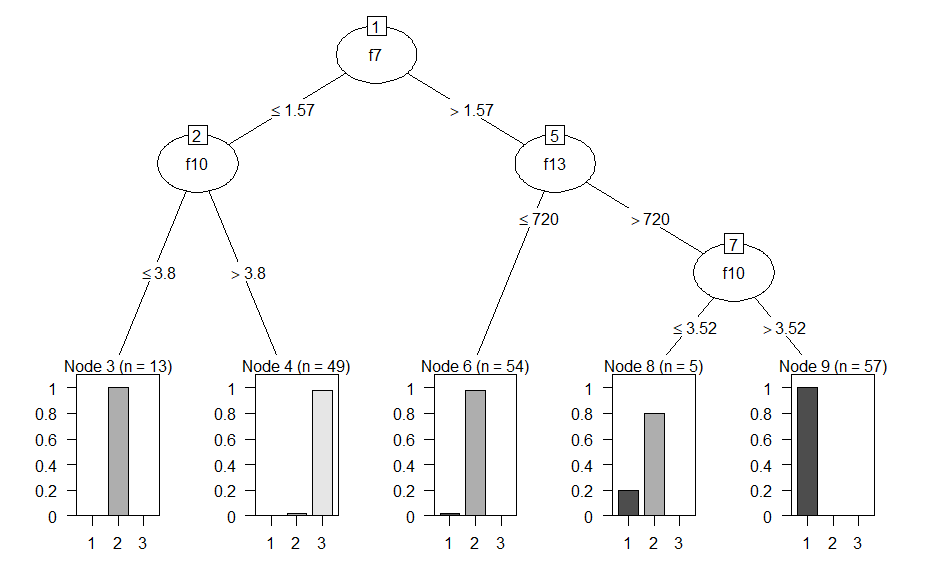
\includegraphics[width=1\textwidth]{wineMinCase5.png}
\caption{Drzewo klasyfikacji instancji wine przy ustawieniu parametru minCases = 5}
\end{figure}

\begin{figure}[H]
\centering
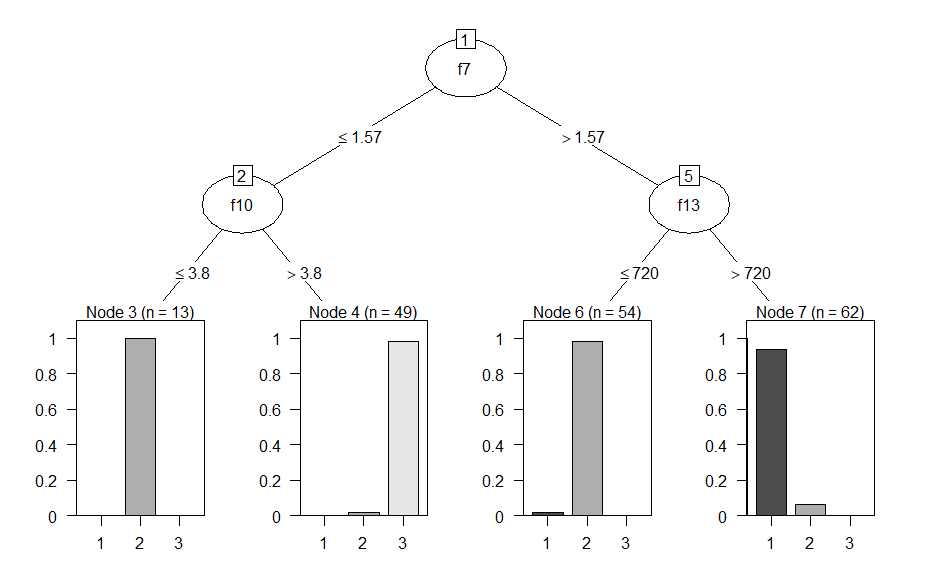
\includegraphics[width=1\textwidth]{wineMinCase10.png}
\caption{Drzewo klasyfikacji instancji wine przy ustawieniu parametru minCases = 10}
\end{figure}

\begin{figure}[H]
\centering
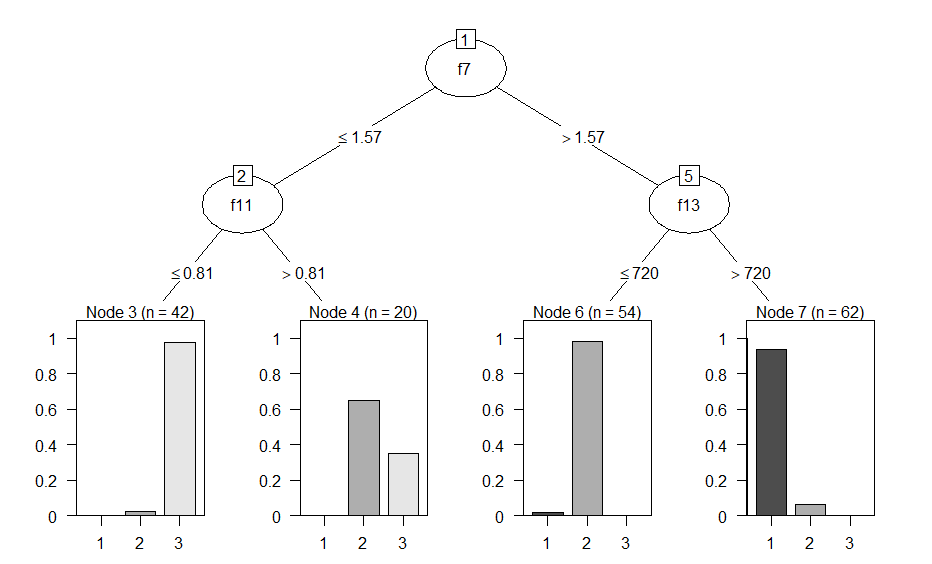
\includegraphics[width=1\textwidth]{wineMinCase20.png}
\caption{Drzewo klasyfikacji instancji wine przy ustawieniu parametru minCases = 20}
\end{figure}

CF - confidence factor - parametr przyjmujący wartość z zakresu <0, 1>. Wraz ze zmniejszeniem wartości, zwiększy się ilość przycinanych węzłów. Pomaga zapobiegać zbyt dużemu rozrostowi drzewa, oraz zjawisku przeuczenia.

\begin{figure}[H]
\centering
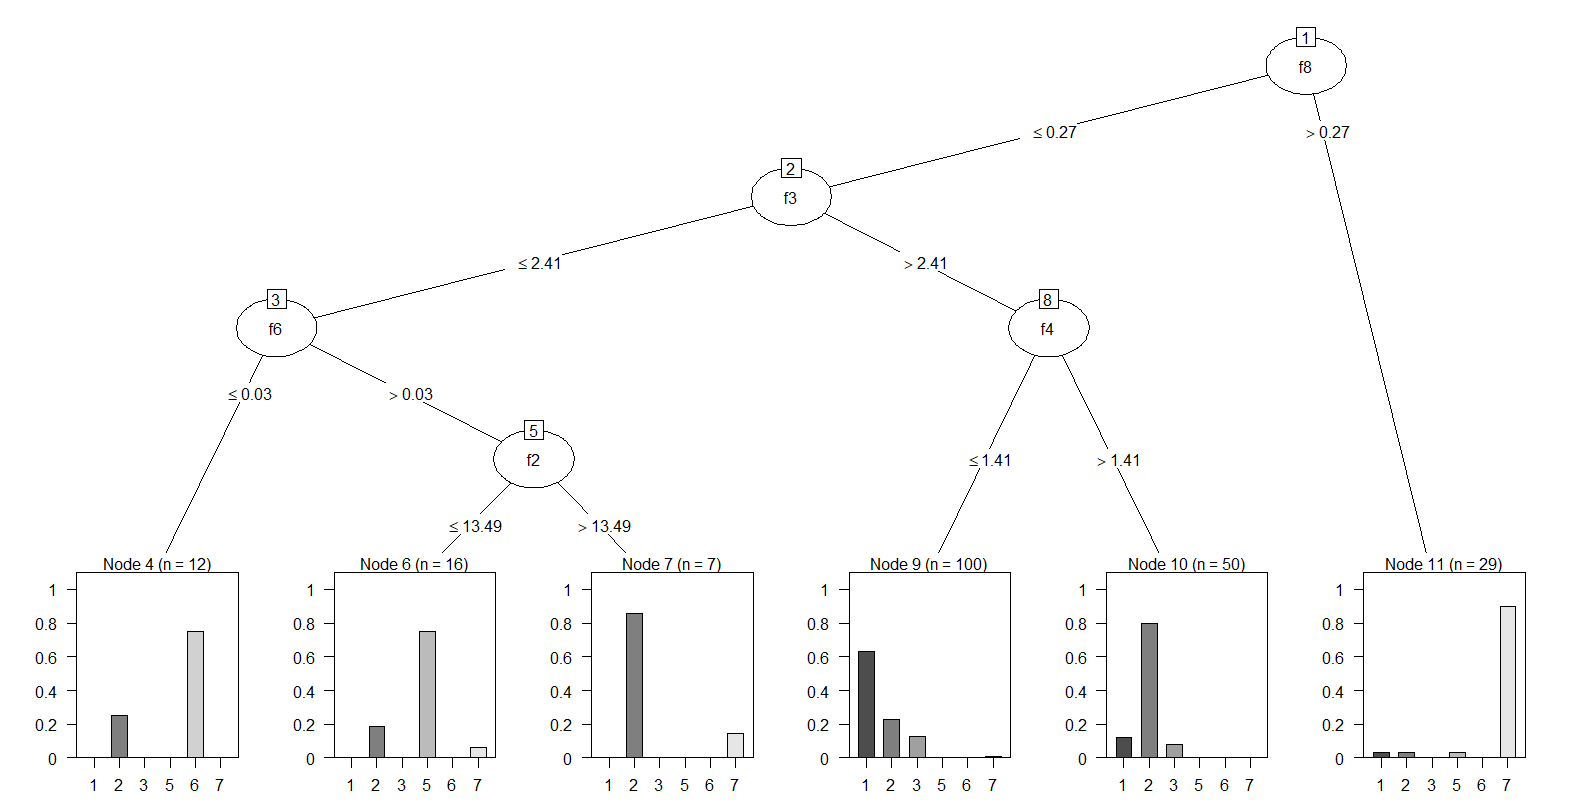
\includegraphics[width=1\textwidth]{glassCF_0.png}
\caption{Drzewo klasyfikacji instancji glass przy ustawieniu parametru CF = 0}
\end{figure}

\begin{figure}[H]
\centering
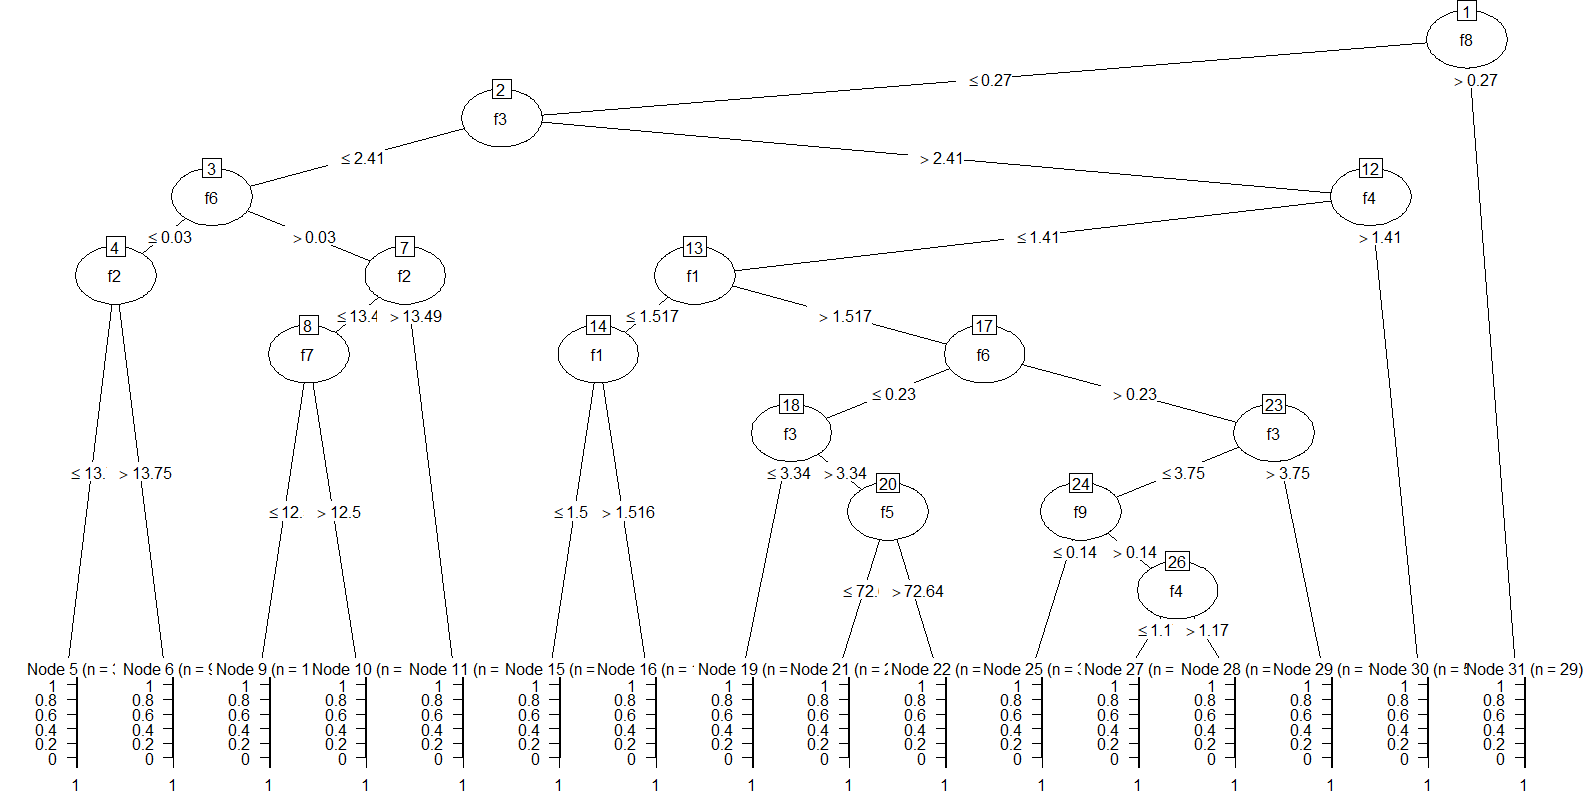
\includegraphics[width=1\textwidth]{glassCF_0_1.png}
\caption{Drzewo klasyfikacji instancji glass przy ustawieniu parametru CF = 0.1}
\end{figure}

\begin{figure}[H]
\centering
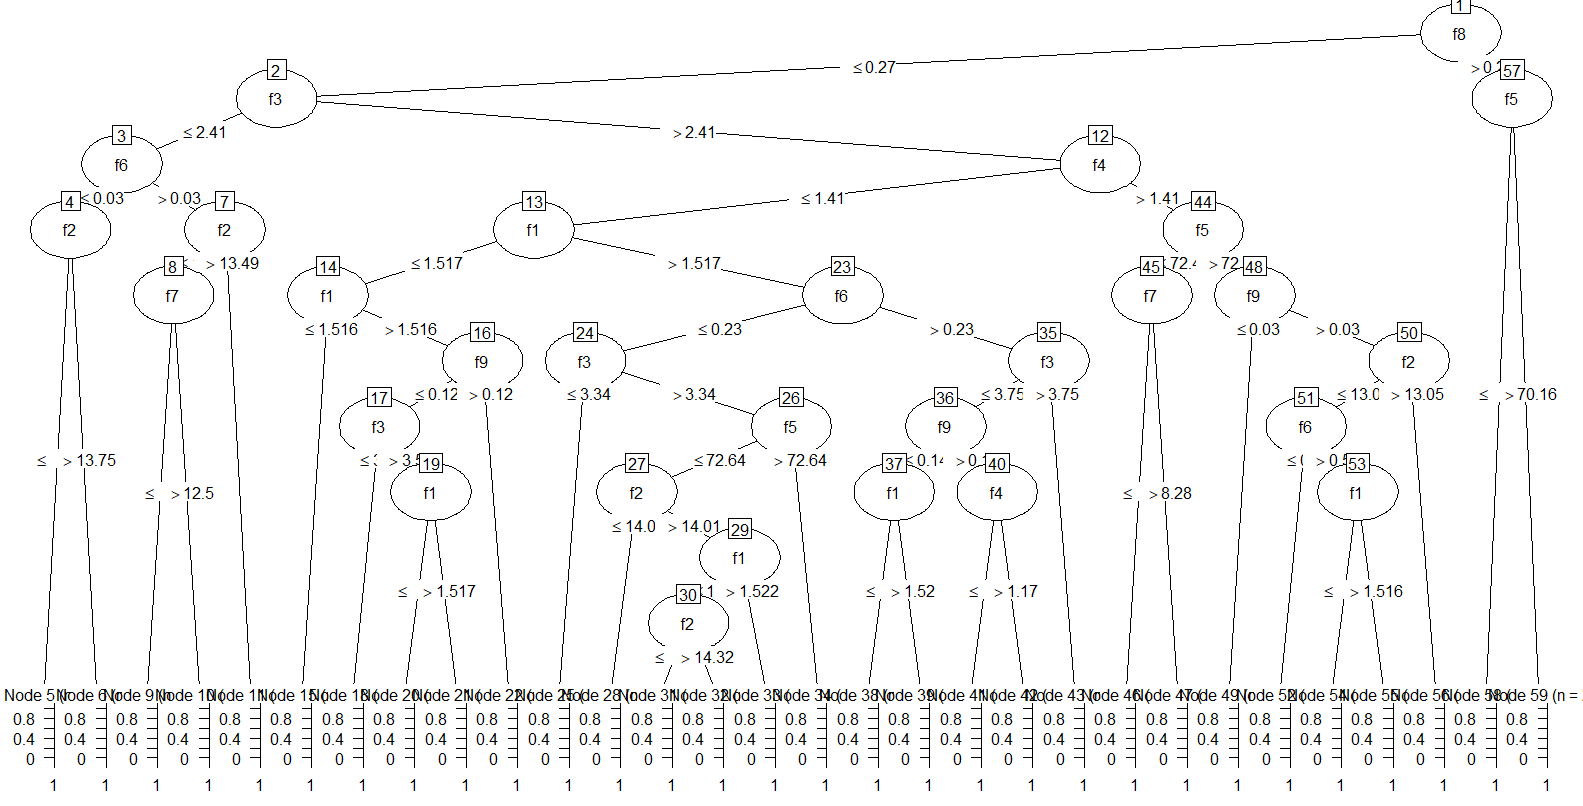
\includegraphics[width=1\textwidth]{glassCF_1.png}
\caption{Drzewo klasyfikacji instancji glass przy ustawieniu parametru CF = 1}
\end{figure}

noGlobalPruning - Przełącznik informujący czy powinien zostać wykonany końcowy krok odpowiedzialny za dodatkowe przycinanie drzewa w celu zmniejszenia jego rozmiaru.

\begin{figure}[H]
\centering
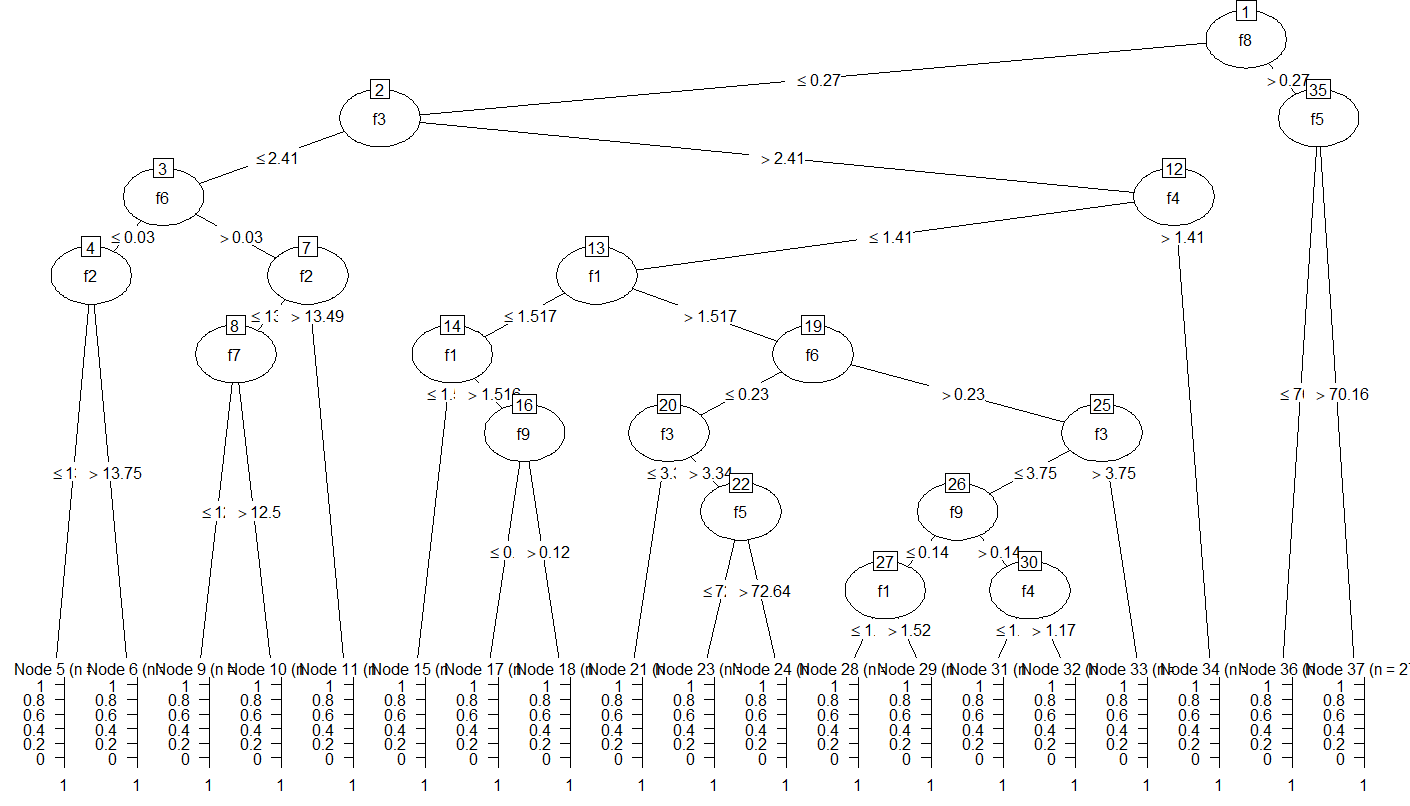
\includegraphics[width=1\textwidth]{no_GP_Glass.png}
\caption{Drzewo klasyfikacji instancji glass przy ustawieniu parametru noGlobalPruning = TRUE}
\end{figure}

\begin{figure}[H]
\centering
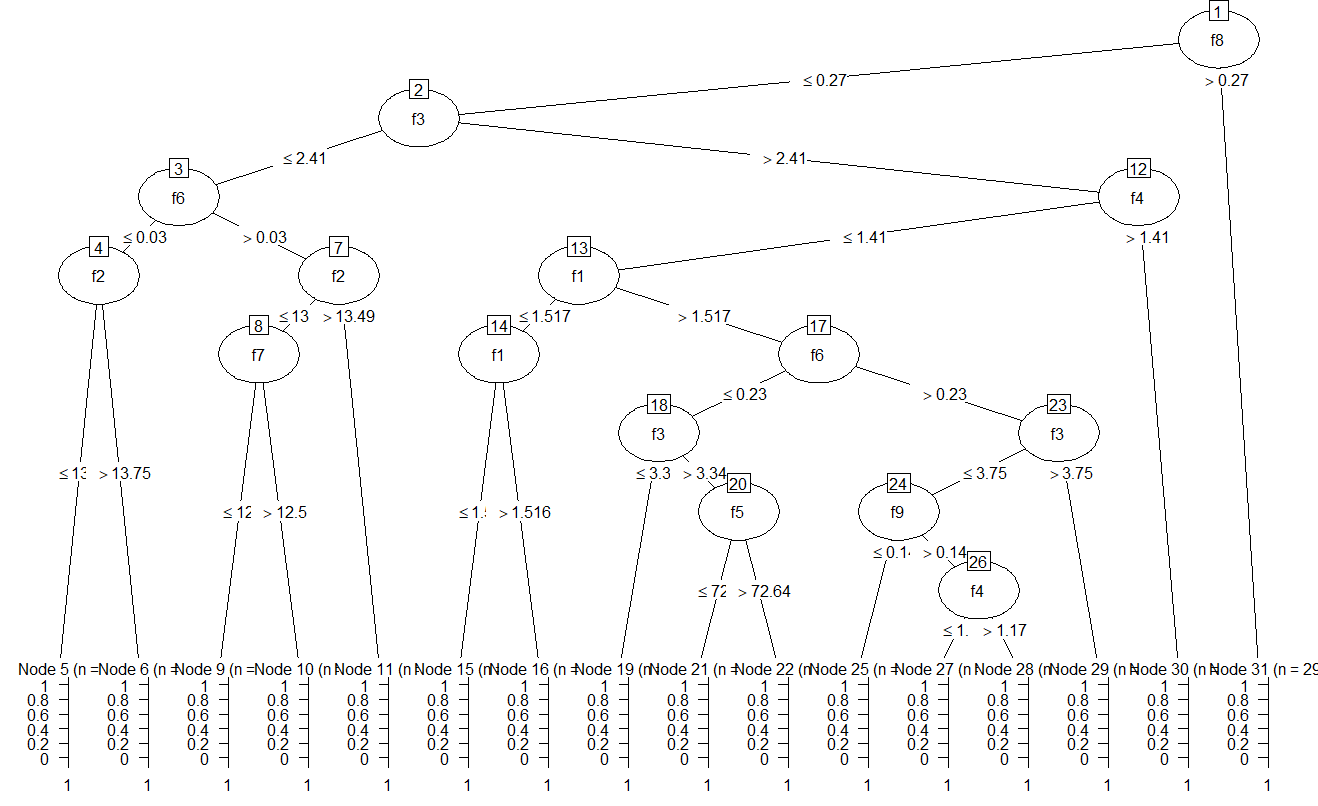
\includegraphics[width=1\textwidth]{GP_Glass.png}
\caption{Drzewo klasyfikacji instancji glass przy ustawieniu parametru noGlobalPruning = FALSE}
\end{figure}

winnowing - Czy powinien zostać zaaplikowany krok przesiewania. Polega on na wstępnej selekcji cech, które mają być wykorzystane do późniejszego modelowania drzewa. Dane zostają rozdzielone na dwie części i dopasowany zostaje inicjacyjny model. Każdy predyktor (przesłanka) jest kolejno eliminowana i sprawdzany jest wpływ takiej operacji na drzewo. Predyktory są oznaczane w zależności od tego czy wpływają one na zwiększenie ilości generowanych błędów.

\begin{figure}[H]
\centering
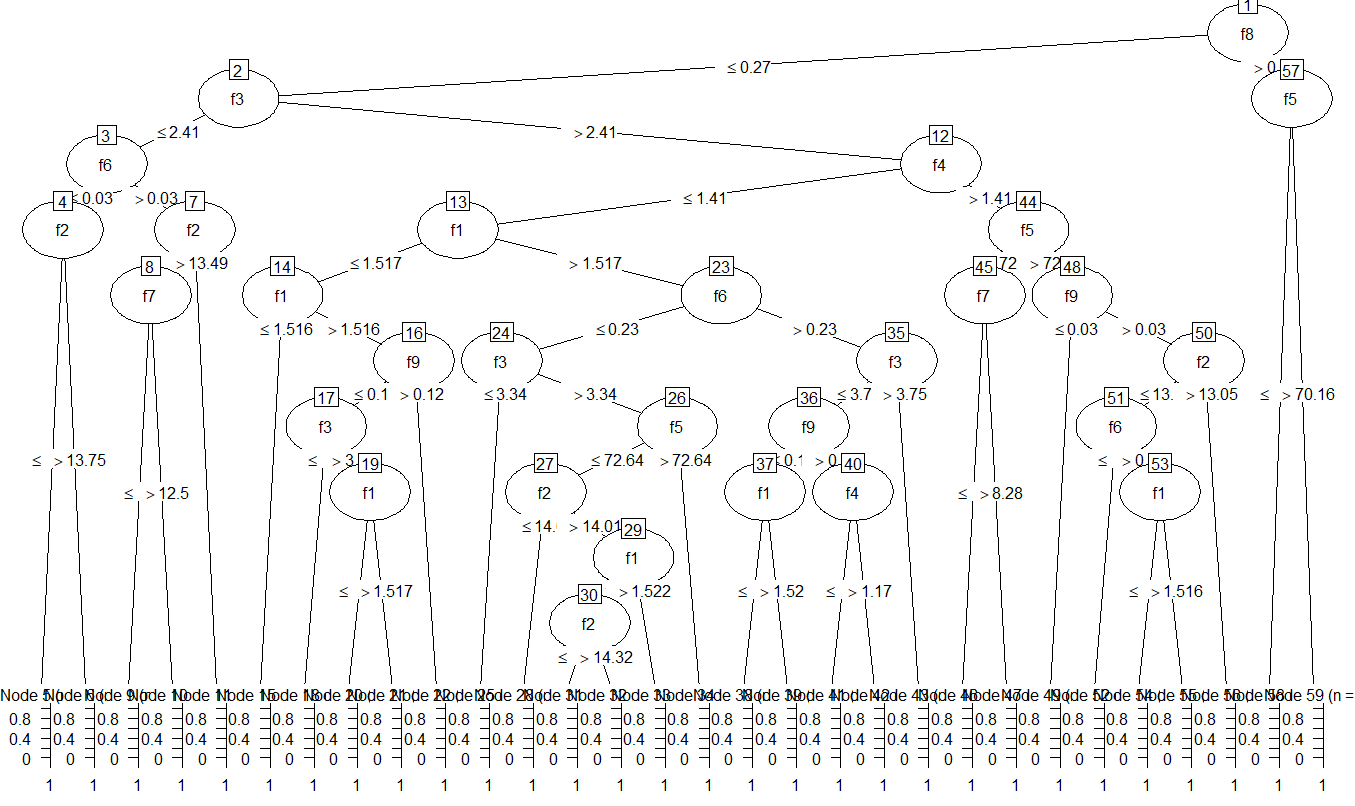
\includegraphics[width=1\textwidth]{glassWinnow_FALSE.png}
\caption{Drzewo klasyfikacji instancji glass przy ustawieniu parametru winnow = FALSE}
\end{figure}

\begin{figure}[H]
\centering
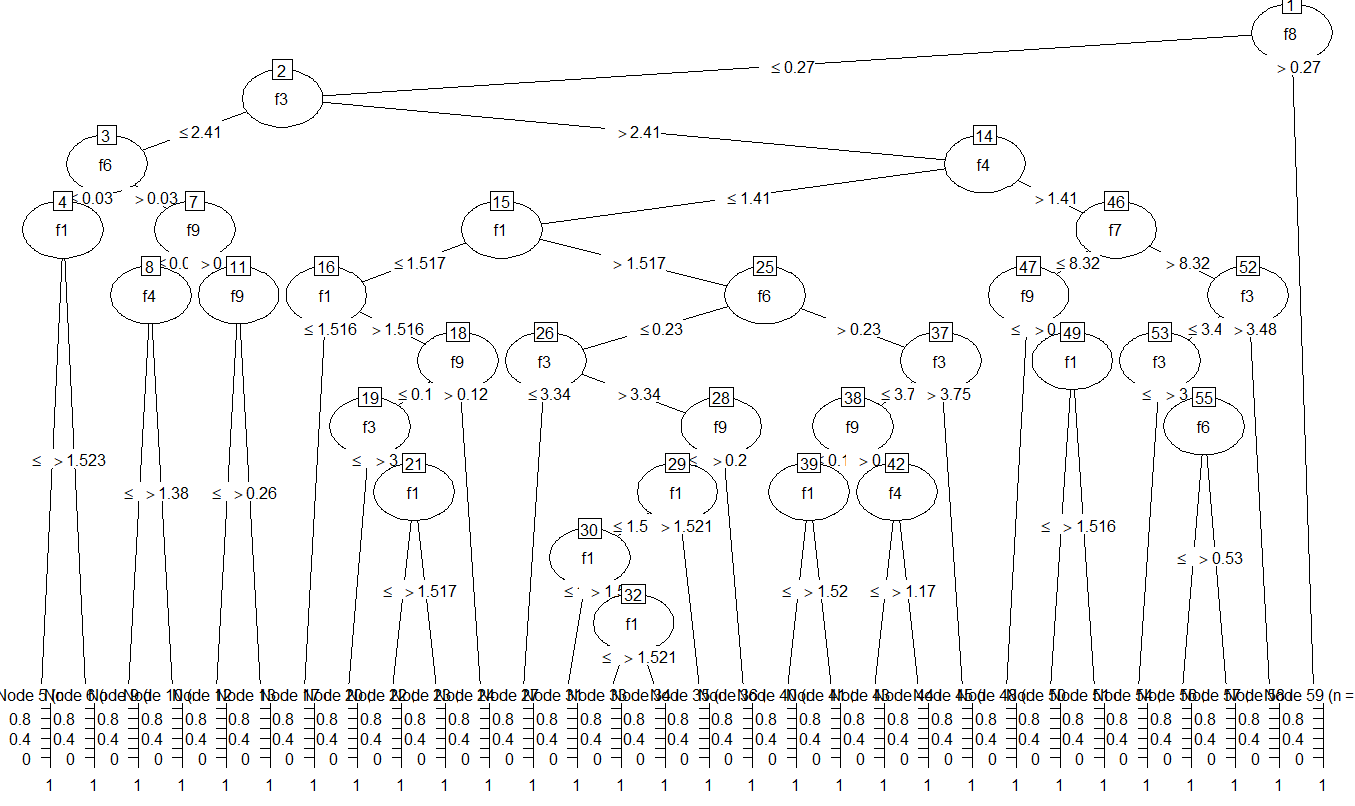
\includegraphics[width=1\textwidth]{glassWinnow_TRUE.png}
\caption{Drzewo klasyfikacji instancji glass przy ustawieniu parametru winnow = FALSE}
\end{figure}

\end{document}